\documentclass{article}
\usepackage{amsmath}
\usepackage{amssymb}
\usepackage[french]{babel}
\usepackage[utf8]{inputenc}
\usepackage[left=.6in,top=1.0in,right=.6in,bottom=1.0in]{geometry}
\usepackage{graphicx}
\graphicspath{{images/}}
\usepackage{subfig}
\usepackage{fancyhdr}
\usepackage{numprint}
\usepackage[boxed]{algorithm2e}
%%%%%%%%%%%%%%%% Lengths %%%%%%%%%%%%%%%%
%\setlength{\textwidth}{15.5cm}
%\setlength{\evensidemargin}{0.5cm}
%\setlength{\oddsidemargin}{0.5cm}

%%%%%%%%%%%%%%%% Variables %%%%%%%%%%%%%%%%
\def\projet{2}
\def\titre{Méthode du gradient conjugué / Application à l'équation de la chaleur}
\def\groupe{1}
\def\equipe{4}
\def\responsible{gdouezangrard}
\def\secretary{rlineatte}
\def\others{sbalafrej, jmarzin, westupin}

%%%%%%%%%%%%%%%% Fancyhdr %%%%%%%%%%%%%%%%
\pagestyle{fancy}
\renewcommand\headrulewidth{1pt}
\fancyhead[L]{\textsc{Projet Algorithmique Numérique}}
\fancyhead[R]{\textsc{Méthode du gradient conjugué / Equation de la chaleur}}
\renewcommand{\footrulewidth}{1pt}
\fancyfoot[L]{\textsc{Enseirb-Matmeca}}
\fancyfoot[C]{\thepage}
\fancyfoot[R]{\textsc{Informatique-1A}}

\begin{document}

%%%%%%%%%%%%%%%% Header %%%%%%%%%%%%%%%%
\noindent\begin{minipage}{\textwidth}
  \vskip 0mm
  \noindent
  {\begin{tabular}{p{7.5cm}}
      {\noindent\bfseries\sffamily{Projet n\textsuperscript{o}}\projet} \\ 
      {\itshape \titre}
    \end{tabular}}
  \hfill 
  \fbox{\begin{tabular}{l}
      {~\hfill \bfseries \sffamily Groupe n\textsuperscript{o}\groupe\ - Équipe n\textsuperscript{o}\equipe
        \hfill~} \\[2mm] 
      Responsable : \responsible \\
      Secrétaire : \secretary \\
      Codeurs : \others
    \end{tabular}}
  \vskip 4mm ~

  ~~~\parbox{0.95\textwidth}{\small \textit{Résumé~:} \sffamily Le but de ce projet consiste à implémenter des algorithmes de résolution de systèmes linéaires de grande taille, et à les appliquer à un exemple de résolution d'équations aux dérivées partielles. Dans ce devoir, nous nous intéresserons aux caractères symétriques, définis positifs et creux de systèmes linéaires, et nous exploiterons ces propriétés pour rendre la résolution plus efficace.}
  \vskip 1mm ~
\end{minipage}

%%%%%%%%%%%%%%%% Main part %%%%%%%%%%%%%%%%
\section{Décomposition de Cholesky}

Dans cette partie, nous nous sommes intéressé à une méthode de factorisation de matrices symétriques : la décomposition de Cholesky.

Cette décomposition consiste à écrire une matrice symétrique définie positive $A$ sous la forme d'un produit ${}^tT.T$ où $T$ est une matrice triangulaire inférieure dont les coefficients sont obtenues par les formules suivantes :

\[\left\lbrace
\begin{array}{lll} t_{i,i} = & a_{i,i} - \sum_{k=1}^{i-1}t_{i,k}^{2} \\
\\
t_{j,i} = & \frac{a_{i,j} - \sum_{k=1}^{i-1}t_{i,k} \cdot t_{j,k}}{t_{i,i}}\,si\,j \geq i
\end{array}\right.\]
\begin{enumerate}

%%%%%%%%%%%%%%%% question 1 %%%%%%%%%%%%%%%%
\item Pour implémenter l'algorithme de factorisation de Cholesky, nous avons choisi de remplir la matrice résultat $T$ colonne par colonne.\\
Chaque terme de la matrice résultat $T$ (triangulaire inférieure) nécessite d'additionner les termes présents sur une même ligne avec un terme de la matrice donnée en entrée. Il faut ensuite diviser par un terme présent dans la diagonale de la matrice $T$.

Il faut donc que ces termes diagonaux soit calculé les premiers pour ne pas faire de divisions par $0$.

En ce qui concerne la complexité, il y a:
\begin{itemize}
\item $\frac{\sum_{k=1}^{n} k^{2}}{2} \sim \frac{n^3}{6}$ additions et multiplications.
\item $\frac{n^{2} - n}{2} = \frac{n \times(n-1)}{2}$ divisions.
\item $n$ racines carrées à calculer.
\end{itemize}

On obtient une complexité en $\Theta(n^3)$ opérations.

%%%%%%%%%%%%%%%% question 2 %%%%%%%%%%%%%%%%
\item La complexité pour résoudre un système linéaire $Ax = b$ correspond à la complexité de la factorisation additionnée à la complexité pour inverser les matrices $T$ et ${}^tT$. On a donc une complexité en $\Theta(n^3)$ opérations (la complexité de l'inversion d'une matrice triangulaire étant négligeable devant celle de la factorisation de Cholesky).

%%%%%%%%%%%%%%%% question 3 %%%%%%%%%%%%%%%%
\item Pour écrire un algorithme permettant de générer des matrices symétriques définies positives creuses avec un nombre de termes extra-diagonaux non-nuls réglable, nous commençons avec une matrice symétrique contenant des termes générés aléatoirement mais distincts de $0$ (générée à partir de la somme d'une matrice et de sa transposée. Pour des raisons de complexité, on évitera le produit matriciel).

Nous identifions alors des positions aléatoires dans la matrice pour lesquelles nous allons placer des $0$ (de façon symétrique bien-entendue, et hors diagonale). Une fois que nous avons placé le nombre de $0$ voulus, nous rendons cette matrice définie positive en calculant en valeur absolue sa valeur propre minimale, puis en ajoutant l'identité multipliée à cette valeur propre (arrondie à l'entier supérieur en valeur absolue). On obtient ainsi une matrice semblable à une matrice diagonale qui n'a que des coefficients strictement positifs (c'est-à-dire les valeurs propre) et elle est donc définie positive.

%%%%%%%%%%%%%%%% question 4 %%%%%%%%%%%%%%%%
\item Les tests à réaliser pour vérifier le bon fonctionnement de cet algorithme consistent à résoudre une équation et vérifier l'exactitude du résultat obtenu grâce à la fonction \verb1linalg.solve1 de Python.

La complexité dans le pire des cas est égale à celle de la factorisation dense. Cependant, plus la matrice sera creuse, plus l'algorithme sera rapide. Il propose cependant des résultats moins précis (voir question 6) que l'algorithme de factorisation dense de Cholesky. Sur le graphe suivant, on peut observer la différence de temps moyenne entre une factorisation dense et une factorisation incomplète pour des matrices ayant quatre termes non-nuls :

\begin{center}
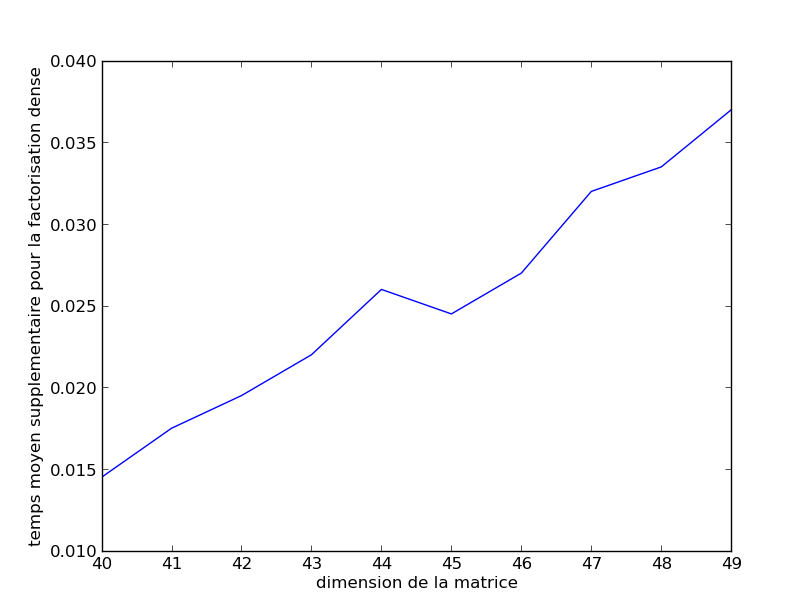
\includegraphics[scale=0.35]{graphemoyenne0.png}
\end{center}


%%%%%%%%%%%%%%%% question 5 %%%%%%%%%%%%%%%%
\item Pour être en mesure d'évaluer le nombre de termes non-nuls gagnés dans le cas de la factorisation dense, nous avons implémenté une fonction qui réalise les deux factorisations (dense et incomplète) sur un nombre fixé de matrices aléatoires et compte le nombre de termes non-nuls obtenus avec chaque méthode. Puis, on compare ces deux nombres et on réalise une moyenne du nombre de termes non-nuls gagnés. Voici un exemple de résultat obtenu grâce à la fonction \verb1graphmoyenne01 :

\begin{center}
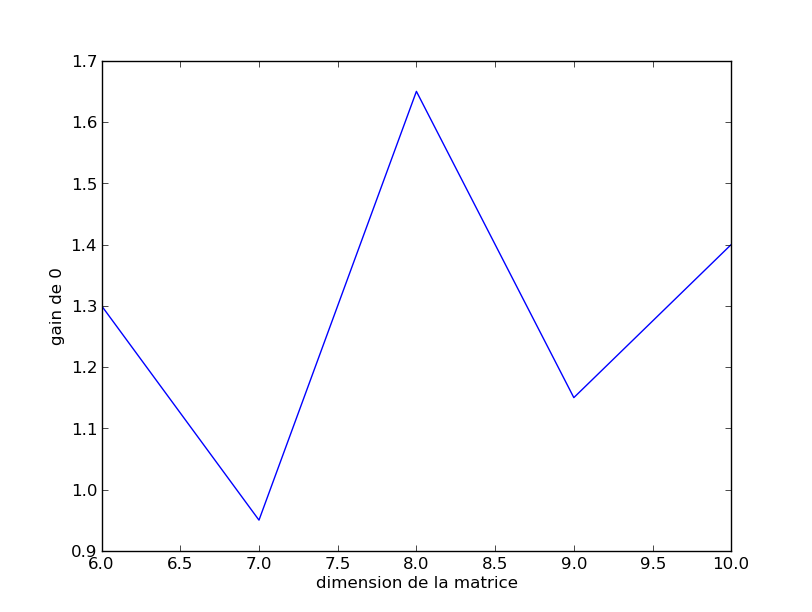
\includegraphics[scale=0.35]{exemple1.png}
\end{center}

Les résultats que l'on obtient sont variables, mais ils permettent d'obtenir une bonne estimation du nombre de termes non-nuls que l'on peut gagner.

%%%%%%%%%%%%%%%% question 6 %%%%%%%%%%%%%%%%
\item À partir d'une matrice A par la factorisation dense de Cholesky, on obtient $A=T{}^tT$.

On a : $M = T {}^tT$.

On en déduit que $\text{cond}(M^{-1}A) = \text{cond}((T{}^tT)^{-1}A) = \text{cond}(A^{-1}A) = \text{cond}(I_n)$

Les préconditionneurs obtenus à l'aide des factorisations de Cholesky  sont très dépendants de la matrice $A$, mais ils permettent de vérifier la relation:
\[\text{cond}(M^{-1}A)\leq \text{cond}(A)\]

Voici, quelques valeurs que l'on obtient avec des matrices de faible dimension:

\begin{center}
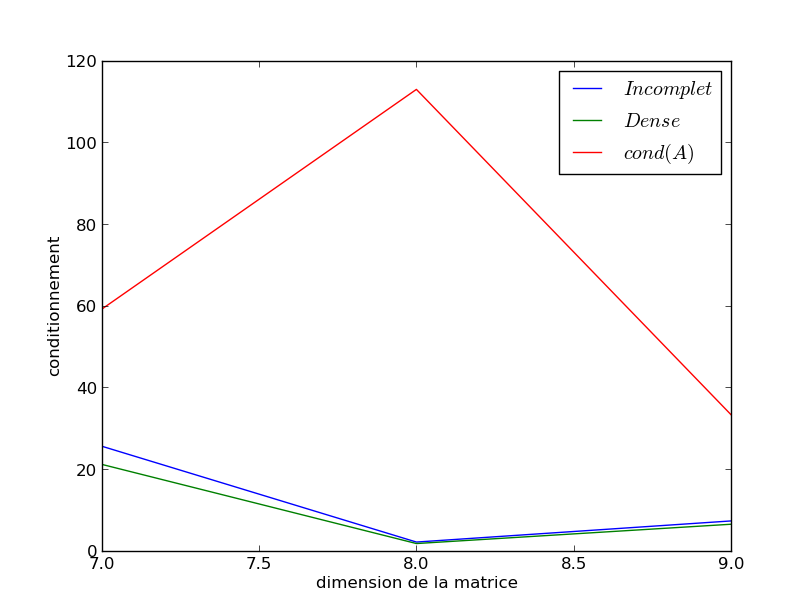
\includegraphics[scale=0.35]{q6.png}
\end{center}

En moyenne, le préconditionneur obtenu à l'aide de la factorisation dense est de meilleur qualité, les résultats sont alors plus précis. Cependant si le nombre de termes nuls dans la matrice est assez important, la factorisation incomplète permet d'obtenir des résultats très proches de ceux que l'on obtient avec la factorisation dense.

Remarque : les résultats obtenus avec les factorisations de Cholesky peuvent être comparés avec ceux donnés par la fonction \verb1linalg.solve1 de Python à l'aide des fonctions \verb1solution_incomplete1 et \verb1solutiondense1 qui renvoient l'erreur relative (ou absolue) pour chaque coordonnée du vecteur résultat.
\end{enumerate}

%%%%%%%%%%%Partie 2 %%%%%%%%%%%%%%%%%%%%%%%%%%%%%%%%%%%%%%%%%%%
\section{Méthode du gradient conjugué}

Dans cette partie, nous nous sommes intéressés à une méthode dite du gradient conjugué. Cette méthode repose sur la convergence du vecteur $x$ vers la solution de l'équation par itération.

\begin{enumerate}
%%%%%%%%%%%%%%Question 1%%%%%%%%%%%%%%%%%%%%%%%%%%%%%%%%%%
\item L'implémentation fournie ne respecte pas certains standard de codages :
\begin{enumerate}
\item L'utilisation d'une boucle \textit{for}, d'un \textit{if} et d'un \textit{break} à la place d'un \textit{while}. L'utilisation de \textit{goto} dans le code n'est pas très saine dans le sens où il sera plus compliqué à debugger, notamment s'il ne s'agit pas de la personne qui a écrit le code.
\item Le nom des variables ne représentent pas très bien ce qu'elles contiennent (bien que nous en ayons conservé les usages pour mieux comparer notre transcription en Python).
\item Il vaudrait mieux utiliser des constantes dans le codes au lieu de nombres (exemple avec le $10^6$ de la boucle for). Nous avons palié à ce problème en définissant des paramètres de fonction optionnels.
\item Dans le code, il n'y a pas de différence entre une matrice de taille $1*1$ et un scalaire, ce qui pose quelques problèmes lors du passage à un language plus exigent, mais peut être intéressant pour des utilisations purement mathématiques.
\end{enumerate}
%%%%%%%%%%%%%Question 2%%%%%%%%%%%%%%%%%%%%%%%%%%%%%%%%%%%%%
\item Cette méthode crée une suite de matrice qui va converger vers la solution de l'équation linéaire. Sa complexité dépend de la taille de la matrice ainsi que de la précision désirée. On a donc une complexité en $\Theta(\log(\varepsilon)*N^2)$.
%%%%%%%%%%%%%Question 3%%%%%%%%%%%%%%%%%%%%%%%%%%%%%%%
\item Nous avons simplement traduit le code matlab en Python.
%%%%%%%%%%%%%Question 4%%%%%%%%%%%%%%%%%%%%%%%%%%%%%%%%%%%%%
\item Nous avons traduit l'algorithme décrit dans le lien du sujet en Python. Nous devons cependant comparer cette méthode avec celle établie précédemment. On constate que l'on obtient un erreur assez élevée en plus de s'exposer rapidemment à un risque de division par $0$...si l'on utilise la formule de Fletcher–Reeves. Mais tout s'arrange dès lors que l'on passe à la formule de Polak–Ribière, et l'algorithme avec préconditionneur s'avère non seulement plus rapide mais bien plus précis (dans la pluspart des cas).
\newpage
Nous avons pu par exemple obtenir cette courbe:

\begin{center}
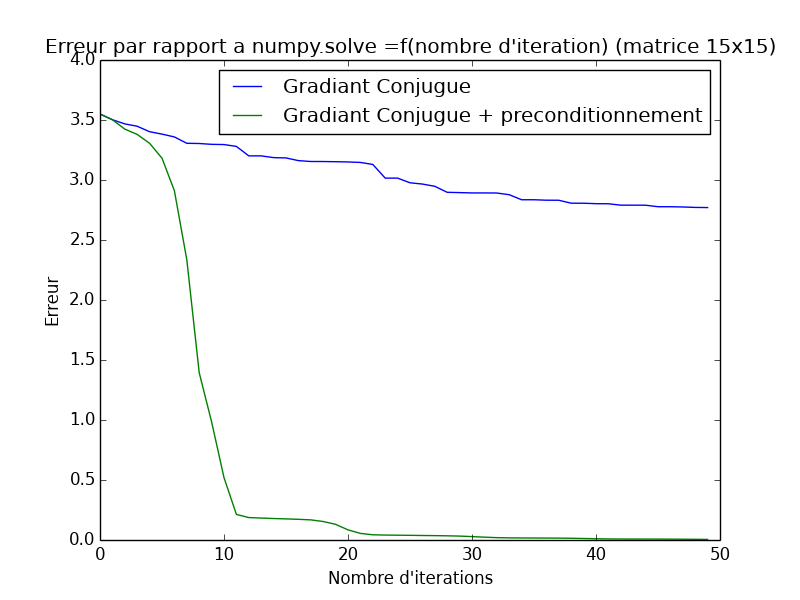
\includegraphics[scale=0.35]{figure_1.png}
\end{center}

A propos des test unitaires, nous n'avons pas eu le temps d'en programmer pour chaque fonction, mais le caractère assez aléatoire de ces algorithmes ne nous permet pas de faire de simples vérifications avec des assert. Nous avons choisi de nous concentrer sur la génération de graphes qui peuvent dans chaque partie être considérés comme des tests des fonctions associées.
%%%%%%%%%%%%%%Fin de la partie 2%%%%%%%%%%%%%%%%%%%%%%%%%%%%%%
\end{enumerate}

%%%%%%%%%%%%%Partie 3%%%%%%%%%%%%%%%%%%%%%%%%%%%%%%%%%%%%%%%%%%
\section{Application à l'équation de la chaleur}

Dans cette partie, nous appliquons les algorithmes vu précédemment à un problème physique : la diffusion de la chaleur dans une pièce.

\begin{enumerate}
%%%%%%%%%%%%%%Question 1%%%%%%%%%%%%%%%%%%%%%%%%%%%%%%%%%%%%%%%
\item Dans en premier temps nous décrivons le problème.

Équation de la chaleur: $T(x,y)$; Température au point $(x,y)$.

\[\frac{\partial^2T}{\partial x^2} + \frac{\partial^2T}{\partial y^2} = f(x,y)\]

Conditions aux limites:
\[T(0,y) = T(1,y) = T(x,0) = T(x,1) = 0\]

Il existe une solution unique au problème.

Nous allons maintenant passer d'un problème continu à un problème discret.

Fixons $N>1$, et on note le point $(x_i,y_j)$.

\[x_i = \frac{i}{N+1}\ ,\ y_j = \frac{j}{N+1}\ \text{pour} (i,j) \in [0,N+1]\]

\[T_{ij} = T(x_i,y_j)\ \text{sont $N^2$ valeurs non nulles.}\]

On va discrétiser les opérateurs différentiels.

\[\frac{\partial T}{\partial x} = \frac{T(x+h,y) - T(x,y)}{h}\]

\[\left(\frac{\partial T}{\partial x}\right)_{ij} = \frac{T(x_i+h,y_j) - T(x_i,y_j)}{h}\]

\[h = \frac{1}{N+1}\ \text{donc}\ \left(\frac{\partial T}{\partial x}\right)_{ij} = \frac{T_{i+1,j} - T_{i,j}}{h}\]

\[et\ \left(\frac{\partial T}{\partial y}\right)_{ij} = \frac{T_{i,j+1} - T_{i,j}}{h}\]

\[\left(\frac{\partial ^2T}{\partial x^2}\right)_{ij} = \frac{(T_{i+1,j} - T_{i,j})-(T_{i,j} - T_{i-1,j}}{h^2} = \frac{T_{i+1,j} + T_{i-1,j} - 2T_{i,j}}{h^2}\]

\[\text{Enfin}\ \left(\frac{\partial ^2T}{\partial x^2} + \frac{\partial ^2T}{\partial y^2}\right) = \frac{T_{i+1,j} + T_{i-1,j} + T_{i,j+1} + T_{i,j-1} - 4T_{i,j}}{h^2} = \Delta T_{ij}\]

On a donc $\Delta T_{ij} = f_{ij}$ un système de $N^2$ équations et de $N^2$ inconnues. On peut donc représenter ce système sous la forme matricielle.

\[-\frac{1}{h^2}M.T = f\]

\[\text{Avec}\ M = \]

    \[\left(\begin{array}{cccc}
    \left(\begin{array}{ccccc|ccccc}
    -4&1&0&0&0&1&0&0&0&0\\
    1&-4&1&0&0&0&1&0&0&0\\
    0&\ddots&\ddots&\ddots&0&0&0&\ddots&0&0\\
    0&0&1&-4&1&0&0&0&1&0\\
    0&0&0&1&-4&0&0&0&0&1\\
    \hline
    1&0&0&0&0&-4&1&0&0&0\\
    0&1&0&0&0&1&-4&1&0&0\\
    0&0&\ddots&0&0&0&\ddots&\ddots&\ddots&0\\
    0&0&0&1&0&0&0&1&-4&1\\
    0&0&0&0&1&0&0&0&1&-4\\
    \end{array}\right)&\ddots\\
    
    \ddots&\left(\begin{array}{ccccc|ccccc}
    -4&1&0&0&0&1&0&0&0&0\\
    1&-4&1&0&0&0&1&0&0&0\\
    0&\ddots&\ddots&\ddots&0&0&0&\ddots&0&0\\
    0&0&1&-4&1&0&0&0&1&0\\
    0&0&0&1&-4&0&0&0&0&1\\
    \hline
    1&0&0&0&0&-4&1&0&0&0\\
    0&1&0&0&0&1&-4&1&0&0\\
    0&0&\ddots&0&0&0&\ddots&\ddots&\ddots&0\\
    0&0&0&1&0&0&0&1&-4&1\\
    0&0&0&0&1&0&0&0&1&-4\\
    \end{array}\right)\end{array}\right)\]
    
%%%%%%%%%%%%%%%Question 2%%%%%%%%%%%%%%%%%%%%%%%%%%

\item Voici le résultat obtenu:

\begin{center}
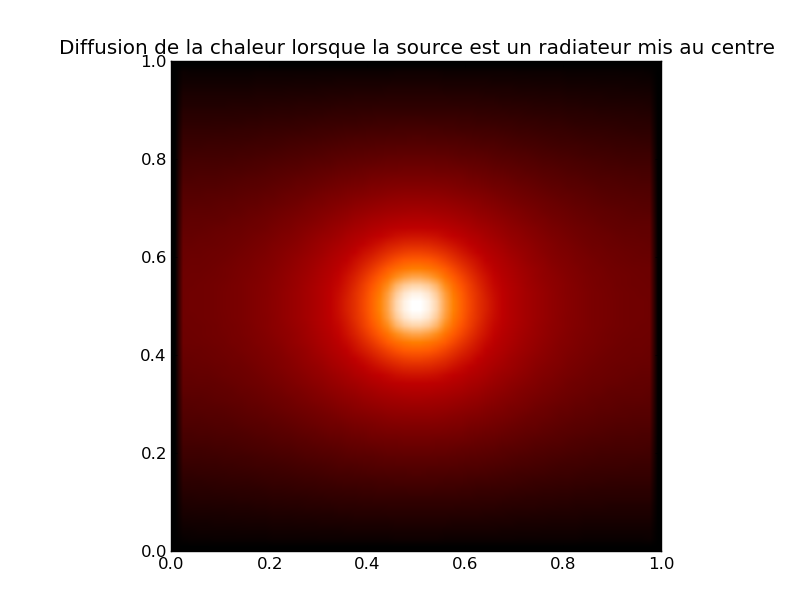
\includegraphics[scale=0.5]{center.png}
\end{center}

On voit bien que la température est la plus importante au centre de la pièce et que la température diminue au fur et à mesure qu'on s'en éloigne.
%%%%%%%%%%%%%%%%%%%%%%%%3%%%%%%%%%%%%%%%%%%%%%%%%
\item Dans le cas d'un radiateur sur le mur, on observe la même graduation de température que le cas précédent mais provenant effectivement du mur.

\begin{center}
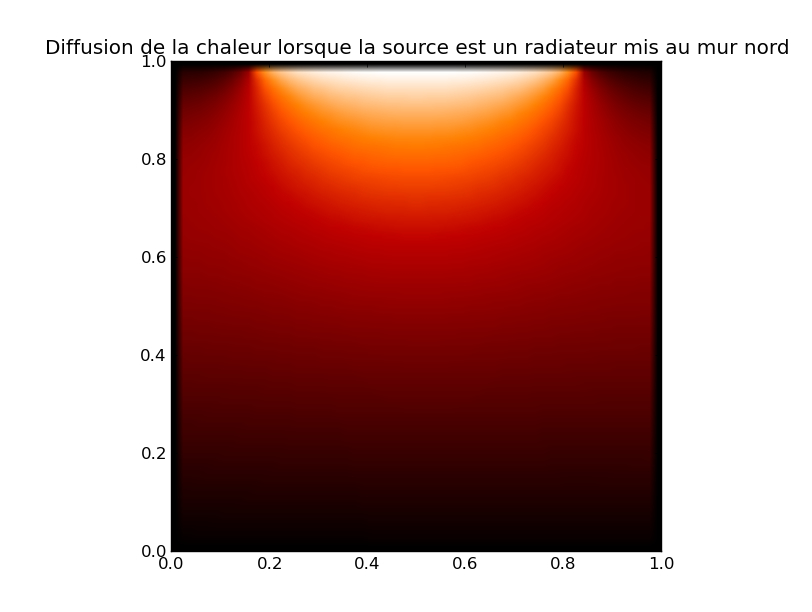
\includegraphics[scale=0.5]{wall.png}
\end{center}
\end{enumerate}

\subsection*{Conclusion}
Ce projet nous a confronté avec un aspect mathématiquement plus solide de l'algorithmique numérique. Nous avons vu un méthode intéressante d'amélioration de la convergence d'un algorithme itératif, par conditionnement, et nous avons pu appliquer ces méthodes à la résolution d'un problème concret qui est l'équation de la chaleur.

\end{document}
